\chapter{Preámbulo.}

\section{Configuración global del documento.}

\section{Paquetes}

\chapter{Contenido.}

\section{Imágenes}

	Lorem ipsum dolor sit amet, consectetur adipiscing elit. Nam viverra sagittis sapien, mollis ornare dolor. Donec fermentum, justo vitae tristique accumsan, urna ex dignissim risus, vitae tempor ante arcu condimentum turpis. Vestibulum tincidunt nulla nec lacus laoreet porttitor. Donec placerat congue mi, cursus dictum dolor viverra vitae. Phasellus venenatis, sapien in congue ornare, augue quam rutrum justo, vel molestie arcu metus luctus urna. Praesent egestas et leo vel ullamcorper. Etiam porta lectus dolor, vitae commodo arcu posuere in. Duis cursus suscipit lacus et tempus. Ut aliquet porttitor tortor in accumsan. Fusce pretium erat non ante tempor ultrices. Donec lorem justo, tincidunt ac finibus sit amet, tempor et dui. Fusce fermentum tempor nisl in blandit. Nam eu neque accumsan, varius tortor in, dictum justo. Ut rutrum tempus tellus, at sollicitudin velit ullamcorper non. In vel velit diam. Sed eu lectus iaculis, porta nisi sit amet, faucibus odio.
	
	Quisque rhoncus sit amet ex id porttitor. Aenean faucibus lectus at leo commodo feugiat. Mauris blandit ipsum non accumsan euismod. Cras nisi nunc, ultricies vel tellus non, ultrices iaculis mauris. Phasellus lorem lorem, cursus nec enim in, porta interdum arcu. Fusce ut imperdiet odio. Sed imperdiet eget enim at pellentesque.
	
	\begin{figure}[H]
		\begin{center}
			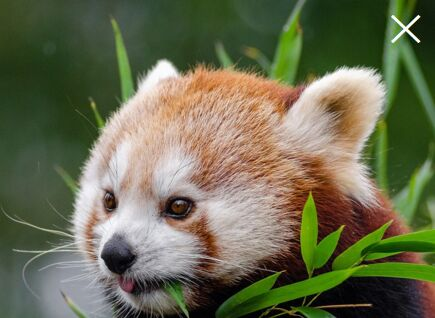
\includegraphics[width = 0.8\GlLineWidth]{rsc/img/TestImage}
			\captionof{figure}{\label{fig:testImgRef}Pie de imagen} 
		\end{center} 
	\end{figure}
	
	Quisque rhoncus sit amet ex id porttitor. Aenean faucibus lectus at leo commodo feugiat. Mauris blandit ipsum non accumsan euismod. Cras nisi nunc, ultricies vel tellus non, ultrices iaculis mauris. Phasellus lorem lorem, cursus nec enim in, porta interdum arcu. Fusce ut imperdiet odio. Sed imperdiet eget enim at pellentesque.
	
	Quisque rhoncus sit amet ex id porttitor. Aenean faucibus lectus at leo commodo feugiat. Mauris blandit ipsum non accumsan euismod. Cras nisi nunc, ultricies vel tellus non, ultrices iaculis mauris. Phasellus lorem lorem, cursus nec enim in, porta interdum arcu. Fusce ut imperdiet odio. Sed imperdiet eget enim at pellentesque.\cite{IEEEreferencias:Ref1} 
	
	Quisque rhoncus sit amet ex id porttitor. Aenean faucibus lectus at leo commodo feugiat. Mauris blandit ipsum non accumsan euismod. Cras nisi nunc, ultricies vel tellus non, ultrices iaculis mauris. Phasellus lorem lorem, cursus nec enim in, porta interdum arcu. Fusce ut imperdiet odio. Sed imperdiet eget enim at pellentesque.\gls{Linux}
	
	
	
\section{Tablas.}
	
	A continuación se muestra una tabla con las siguientes características
	\begin{itemize}
		\item Ancho igual al del texto.
		\item Se expecifica la alineación de las columnas
		\item Incluye un texto al pie de la tabla y una etiqueta para poder hacer referencia \ref{tab:tabularx_simple}.
	\end{itemize}
	
%	\begin{table}[H]
%		\begin{tabularx}{\textwidth}{|c|X|}
%			\hline 
%			\textbf{Núm. de pin} & \textbf{Descripción} \\ \hline 
%			1. GND & Se conecta a nuestra referencia de 0 \si{\volt} \\ \hline 
%			2. TX & Se conecta al pin RX de nuestra interfaz para configurar el módulo \\ \hline 
%			4. ENB & Se conecta a nuestro voltaje de alimentación de 3.3 \si{\volt} \\ \hline 
%			7. RX & Se conecta al pin RX de nuestra interfaz para configurar el módulo \\ \hline 
%			8. VCC & Se conecta a nuestro voltaje de alimentación a 3.3 \si{\volt}  \\ \hline 
%		\end{tabularx}
%		\caption{\label{tab:simple_tabularx} Pines que deberán conectarse al módulo para configurarlo.}
%	\end{table}
%	
%	También se pueden alinear las columnas como en la tabla \
%	
%	\begin{table}[H]	
%		\centering		
%		\begin{tabularx}{0.5\textwidth}{
%				|>{\raggedright\arraybackslash}X
%				|>{\centering\arraybackslash}X
%				|>{\raggedleft\arraybackslash}X|}
%			\hline 
%			$\phi$ & $\psi$ & $\phi\wedge\psi$ \\ \hline 
%			T & T & T \\ \hline 
%			T & F & F \\ \hline 
%			F & T & F \\ \hline 
%			F & F & F \\ \hline 
%		\end{tabularx} 
%		\caption{\label{tab:tabularx_align} Tabla de verdad proposicional. }
%	\end{table}
%	
%	\begin{tabularx}{0.7\textwidth}{
%			|>{\raggedright\arraybackslash}X
%			|>{\centering\arraybackslash}X
%			|>{\raggedleft\arraybackslash}X|
%	}
%		\hline
%		\multicolumn{1}{|c}{Título 1} & \multicolumn{1}{|c}{Título 2} & \multicolumn{1}{|c|}{Título 3} \\ \hline 
%		Contenido izquierda, contenido a la izquierda, contenido a la izquierda & Contenido izquierda & Contenido izquierda \\ \hline 
%		Más texto & Más texto & Más texto\\ \hline 
%	\end{tabularx}
	


	\begin{table}[H]
		\centering
	\begin{tblr}{
			width = 0.7\textwidth,
			colspec = {|X[l,m]|X[c,m]|X[r,m]|}, % Definimos la alineación en la especificación de columnas
			hlines,
			vlines,		
			rows = {m},
			row{odd} = {bg=gray!30},
			%row{even} = {bg=red!30},
			row{1} = {font=\bfseries, bg=gray!60, c}, % La primera fila centrada
		}	
		Encabezado 1 & Encabezado 2 & Encabezado 3 \\ \hline
		Texto izquierda & Texto centrado & Texto derecha \\
		Más contenido largo, más contenido largo, más contenido largo. & \colorbox{light-Green}{$\phi$} & 12345 \\
		Otro texto & \textcolor{Red}{texto} & Final	\\
		Texto izquierda & Texto centrado & Texto derecha \\
		Línea 1 \linebreak Línea 2 \linebreak Línea 3 & 
		Línea 1 \linebreak Línea 2 \linebreak Línea 3 & 
		Línea 1 \linebreak Línea 2 \linebreak Línea 3 \\		
		
	\end{tblr}
	\caption{\label{tab:simple_tabularx} Pines que deberán conectarse al módulo para configurarlo.}
	\end{table}

	
%	\begin{tblr}{
%			width = \textwidth,
%			colspec = {|X[c,m]|X[c,m]|X[c,m]|},
%			hlines,
%			vlines,
%			row{1} = {font=\bfseries, bg=lightgray},
%			rows = {m}, 
%			cell{2-last}{1} = {l},
%			cell{2-last}{3} = {r},
%			row{even} = {bg=lightgray!20}
%		}
%		Encabezado 1 & Encabezado 2 & Encabezado 3 \\
%		Texto izquierda & Texto centrado & Texto derecha \\
%		Más contenido & Con varias líneas & 12345 \\
%		Otro texto & Centrado & Final
%	\end{tblr}
	
	
	
	
	

	
	Vestibulum sollicitudin imperdiet nisl. Nullam eget nisi nunc. Quisque eget accumsan lorem, nec interdum neque. Pellentesque habitant morbi tristique senectus et netus et malesuada fames ac turpis egestas. Vestibulum ante ipsum primis in faucibus orci luctus et ultrices posuere cubilia Curae; Nullam at metus dignissim, euismod diam in, maximus sem. Sed semper rhoncus lectus eu tempor.
	
	Vestibulum sollicitudin imperdiet nisl. Nullam eget nisi nunc. Quisque eget accumsan lorem, nec interdum neque. Pellentesque habitant morbi tristique senectus et netus et malesuada fames ac turpis egestas. Vestibulum ante ipsum primis in faucibus orci luctus et ultrices posuere cubilia Curae; Nullam at metus dignissim, euismod diam in, maximus sem. Sed semper rhoncus lectus eu tempor.
	
	Vestibulum sollicitudin imperdiet nisl. Nullam eget nisi nunc. Quisque eget accumsan lorem, nec interdum neque. Pellentesque habitant morbi tristique senectus et netus et malesuada fames ac turpis egestas. Vestibulum ante ipsum primis in faucibus orci luctus et ultrices posuere cubilia Curae; Nullam at metus dignissim, euismod diam in, maximus sem. Sed semper rhoncus lectus eu tempor.
	
	\section{Sección 3}
	
	Phasellus bibendum dignissim efficitur. Vestibulum venenatis leo in lorem blandit dignissim. Praesent scelerisque dapibus lectus vel efficitur. Fusce tristique nulla at tempor eleifend. Vivamus ullamcorper volutpat lorem. Integer sodales molestie cursus. Aliquam felis mi, ultricies nec ante a, tincidunt semper nulla. In convallis finibus nibh id ultrices.

	\section{Sección 4}
	Quisque ligula ex, semper eu tristique sit amet, accumsan vitae eros. Proin sodales hendrerit metus sit amet tincidunt. Etiam dictum cursus tellus id malesuada. Integer accumsan augue eu lectus consectetur, vel interdum turpis posuere. Pellentesque pellentesque lacinia enim, semper consectetur sem lacinia in. Etiam bibendum tristique justo ac blandit. Curabitur vitae dapibus odio, tempus ornare dolor. Maecenas dui urna, luctus at auctor at, tincidunt non eros. Proin euismod, lacus nec faucibus congue, orci magna vulputate est, quis tempus orci urna eget justo. Nulla a placerat turpis.
